\documentclass[tikz,border=5pt]{standalone}
\usepackage{pgfplots}
\pgfplotsset{compat=1.18}

\definecolor{corba}{HTML}{365FB3}
\definecolor{punt}{HTML}{B91C1C}
\definecolor{assimptota}{HTML}{6B7280}

\begin{document}
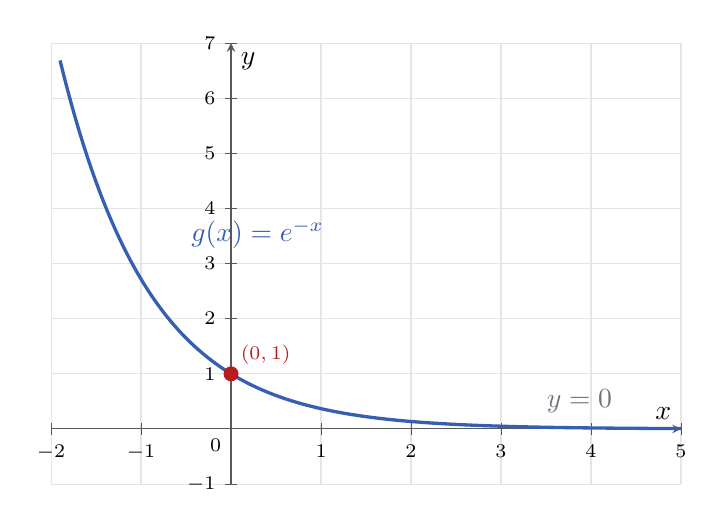
\begin{tikzpicture}
  \begin{axis}[
    width=8cm,
    height=5.6cm,
    scale only axis,
    axis lines=middle,
    grid=major,
    grid style={black!10},
    axis line style={black!65},
    tick style={black!65},
    tick label style={font=\scriptsize},
    xlabel={$x$},
    ylabel={$y$},
    xmin=-2, xmax=5,
    ymin=-1, ymax=7,
    xtick={-2,-1,0,1,2,3,4,5},
    ytick={-1,0,1,2,3,4,5,6,7},
    clip=false,
  ]
    \addplot[corba, very thick, domain=-1.9:5, samples=240]
      {exp(-x)};
    \addplot[only marks, mark=*, mark size=2.5pt, punt]
      coordinates {(0,1)};
    \node[anchor=north east, font=\scriptsize]
      at (axis cs:0,0) {$0$};
    \node[anchor=south west, text=punt, font=\scriptsize]
      at (axis cs:0,1) {$(0,1)$};
    \node[anchor=south west, text=assimptota]
      at (axis cs:3.4,0.12) {$y=0$};
    \node[anchor=south west, text=corba]
      at (axis cs:-0.55,3.1) {$g(x)=e^{-x}$};
  \end{axis}
\end{tikzpicture}
\end{document}
